\documentclass[12pt,letterpaper,onecolumn,twoside]{article}
\usepackage[spanish]{babel}
\usepackage[left=2cm,right=2cm,top=1.5cm,bottom=1.5cm]{geometry}
\usepackage{fancyhdr}
\pagestyle{fancy}
\fancyhead{}\lhead{}\chead{}\rhead{}
\renewcommand{\headrulewidth}{0pt}
\usepackage[latin1]{inputenc}
\usepackage{amsmath}
\usepackage{graphicx} % gr�ficos
\usepackage{subfigure} % subgr�fico
\usepackage{lscape}
\usepackage{setspace}
\usepackage{enumitem}
\usepackage[noblocks]{authblk}
\usepackage{float}
\usepackage{cite}% para contraer referencias
\usepackage[usenames]{color}
\providecommand{\abs}[1]{\lvert#1\rvert}
\providecommand{\norm}[1]{\lVert#1\rVert}
 \title{\textbf{Optimization of Porous Silicon (PSi) with gradient refractive index (GRIN): A comparison with computational schemes with experimental results } }

\author[1]{C. A. Ospina de la Cruz}
\author[2]{W. L. Mochan }
\author[3]{V. Agarwal }

\affil[1]{{\scriptsize Posgrado en Ingenier\'ia y Ciencias Aplicadas del Centro de Investigaci�n en Ingenier\'ia y Ciencias Aplicadas (CIICAp-IICBA), Universidad Aut�noma del Estado de Morelos (UAEM), Cuernavaca CP 62209, M�xico}}
\affil[2]{{\scriptsize Instituto de Ciencias F\'isica ,Universidad Nacional Autonoma de Mexico, Av. Universidad S/N, Col. Chamilpa, 62210 Cuernavaca, Morelos, Mexico  } }
\affil[3]{{\scriptsize Centro de Investigaci\'on en Ingenier\'ia y Ciencias Aplicadas,Universidad del Estado de Morelos, Av. Universidad 1001 Col. Chamilpa, Cuernavaca, Morelos 62209, Mexico  } }
\affil[*]{{\scriptsize Corresponding author: xxxxxx@xxxx.xxx}}
\date{}

\begin{document}
\renewcommand{\contentsname}{Contents}
\renewcommand{\abstractname}{Abstract}
\renewcommand{\tablename}{Table}
\vspace{50pt}

\maketitle
\begin{abstract}
The current density in a of Porous Silicon (PSi) with gradient  refractive index (GRIN) produced  by an electrochemical  attack on silicon (Si)  to  produce  porous  silicon (PSi), the calculated  porosity  of the GRIN structure depends  on the  position  and  distance  from  counter  electrode.   The proposed relationship shows, the  counter  electrode tip that acts  analogously  as a point charge  and  current density  for a geometry in an electrolytic  box by solving the electrostatic equations  with suitable  contour conditions.  Resulting  in an electrostatic model for photonic  crystals  with gradient refractive index (EMPCGRIN). The characterization of the  silicon structures was performed  by scanning electron microscopy   and  UV-Vis-NIR reflectance spectroscopy.  The obtained  results  open  the  possibility  of creating  silicon-based photonic  structures within  the  Visible-IR- range, within  the  sample at  different measuring distances,  where generally porous silicon does not strongly  absorb or disperse light.  Similarly, in the UV-Visible range  there is a strong absorption with more of light scattering. Having a greater  area of attack generating  different pores sizes and their porosity, and making an easy calculation  in the manufacture of porous silicon. \\

Keywords: Porous Silicon (PSi); Monolayer(Ml); Porosity(P); Reflectance Spectra.
\end{abstract}


\vspace{-0.8cm}
\singlespacing
\tableofcontents

%\newpage
\spacing{1}


 \section{Introduction}

 The structural behavior of nanostructured materials  has  become a  great  topic  of global  interest,  where numerous  research has been done so far \cite{I1}. We found a great way to go for future technological  explorations,  countless  challenges and  that  open a range of possibilities to develop further  study  on these issues\cite{I2}. Porous silicon (PSi) is a versatile nanostructured material and an excellent candidate as a technological platform for different sensing applications \cite{I3, I4}, due to its easy manufacturing,  large surface area, high surface reactivity,  and moreover, its optical transduction capacity.  Photonic crystals are multilayer dielectric structures that have periodicity in the dielectric function along one direction \cite{I5}. It has numerous studies for high reflectivity and the ability to adjust  the photonic  prohibited  band (PBG)\cite{I6} , which leads to possible applications  such as filters\cite{I7}, optical switches\cite{I8}, omnidirectional mirrors\cite{I9}, waveguides for PC \cite{I10} etc. In the conventional manufacturing of PSi the desired result  is to obtain  homogeneous samples (same structural characteristics) from the  periphery  to the center  of the electrochemically  attacked area.  However, with an asymmetric anodizing configuration,  samples with a lateral gradient in terms of pore size and thickness of the porous layer are obtained \cite{I101}. In this configuration,  the face of the platinum  electrode (cathode)  is relatively maintained  perpendicular  to the surface of the Si substrate (anode) at one end of the cell, so that the distribution of the current within the electrolyte  solution varies depending on the distance  of the electrode due to the resistance of the electrolyte,  resulting  in a decrease in current density as the distance from the electrode increases \cite{I102, I103}. The result is a porous surface with different pore sizes ranging from a few nanometers  to pores on the order of a few micrometers  \cite{I104}. The dimensions of the pores obtained on the same chip can be controlled by adjusting the anodizing current and electrolyte concentration \cite{I11}. Currently, these types of samples have found their application relevant as optical band filters \cite{I12}, devices with a multidirectional photonic band (photonic bar codes) \cite{I13} and mainly as biosensors. In this way, the effect of different topographies (porosities in the same sample) on the culture / adhesion of certain cells \cite{I14} is studied, considerably reducing the number of samples and cost of the study. In addition, they are also very useful when a biomolecule size-exclusion technique is required allowing the identification and separation of these biological compounds \cite{I15}. Recent studies  have shown that  the  combination  of thermal  oxidation  and infiltration of TiO2   by ALD offers the  opportunity to manufacture  a high index of refraction  of contrast, visibly transparent GRIN optical elements from PSi absorbent structures \cite{I16}. A Despite previous research on the formation of porous silicon with GRIN, type p in manufacturing and characterization, there was no control of current densities, much less a model that  explained said lateral  gradient. In this work, we reported a gradient refractive index (GRIN) structure by varying the current density on the fabrication of porous silicon photonic structure. This current density values, depth, and porosity of the photonic structure were calculated from an electrostatic model for photonic crystals with a gradient refractive index (EMPCGRIN). Moreover, the theoretical and experimental studies were exhibited similar results.\\
 The paper is organized as follows. In Section 2  we report the effect of how the current density can be calculated from an electrostatic model for photonic crystals with gradient refractive index (EMPCGRIN), demonstrating that there is a direct relation of the gradient generated by the electrode when it attacks the Silicon sample, we can see the depth of the structure and its porosity, in each of the measuring points. In Subsection 2.2 we present a formalism based on the methods used for the analysis of photonic crystal structures is the transfer matrix method. We use it to investigate the reflectance of light in a one-dimensional photonic crystal. In Section 3 we provide experimental  details about the manufacture of PS dielectric multilayers and Section 4 we shows the comparison of numerical and experimental results followed. Finally,  the conclusions given in Section. 5

 \section{Theory}
 \subsection{Electrostatic Model for Photonic Crystals with Gradient Refraction Index (EMPCGRIN)}
The calculate  current density in a GRIN structure produced by an electrochemical attack on Si to produce Porous Si with a position-dependent porosity due to the distance to the counter electrode. A simplifies  calculation  with geometry,
assumimg  in the form of a whole prism on the sides a, b, c with a, b horizontal and c vertical. Here c considered as the height of the liquid, and the walls are insulating, but the bottom is completely covered with the sample, which act as good conductor. The electrode is a thin insulated cable with tip, which  a point  current source.
\begin{figure}[H]
	\centering
	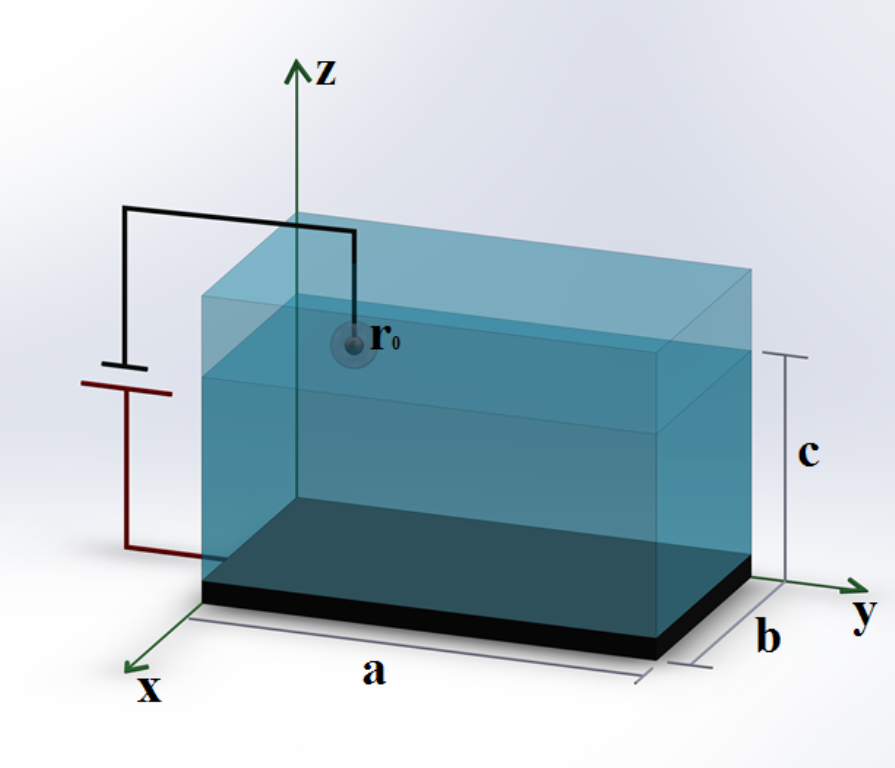
\includegraphics[scale=.4]{../Images/celdan}
	\caption{\emph{Diagram of the Electrolytic cell where we can see the shape of a prism on the sides a, b, c with a, b horizontal and c vertical. I'll take as the height of the liquid. The walls are insulating, but the bottom is completely covered by the sample, I suppose it is a good conductor. The tip of the electrode is a thin insulated wire located at $ \vec{r}_0 $.}}
\end{figure}
The current in the electrolyte is $ \vec {J} = \sigma \vec{E} $ with $ \sigma $ is the conductivity. This for the stationary case $ \bigtriangledown \cdot \vec{j} = 0 $. The electric field is derived from the electric potential, $\vec {E} = - \bigtriangledown \varphi $.
And we can say that $ \bigtriangledown^{2} \varphi = 0 $, since the sample is a relatively good conductor, when connected to earth $ \varphi(x, y, 0) = 0 $. Integrating $ \vec{J} $ over a small sphere superimposing the electrode gives $ \int ds \cdot \vec{J} = I $.
The current density that carries the current to the tip. So
  \begin{equation}
\int ds \cdot \vec{E} = \dfrac{I}{\sigma}
\end{equation}
The problem to be solved is thus, to obtain the potential produced by a point charge,
  \begin{equation}
 q_{_{0}} = \dfrac{I}{4 \pi \sigma}
 \end{equation}
In the positions$\vec{r}_{_{0}}=(x_{_{0}}, y_{_{0}}, z_{_{0}})$ is the tip of the electrode that is in the presence of a ground conductor plane grounded $ z = 0 $ and enclosed on the insulating walls at $ (0, y, z) $, $ (a, y, z) $, $ (x, 0, z) $ , $ (x, b, z) $. The surface of the liquid is also not conductive to $ (x, y, c) $, the normal current is $\vec{j} \cdot \hat{n}=0$ and the normal of the field is $ \vec{E} \cdot \hat{n}=0  $. i.e
\begin{equation}
E_{_{x}}(0, y ,z)= E_{_{x}}(a, y ,z)=E_{{_y}}(x, 0 ,z)=E_{{_y}}(x, b ,z)=E_{{_z}}(x, y ,c)=0
\end{equation}
This has a mixture of Dirichlet-Neumann type boundary conditions. By using the simplified prism geometry  can solve the problem using the theory of image loads. Each load has an image of the same sign and magnitude for each lateral insulating surface and the opposite sign change in the lower part of the conductive plane, as follows.
 \begin{figure}[H]
 \centering
 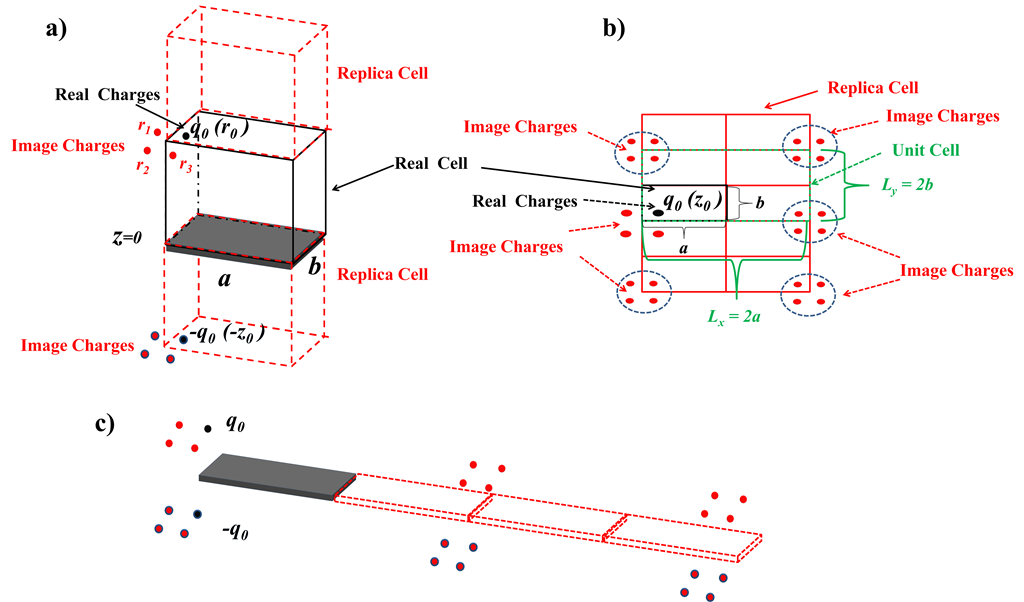
\includegraphics[scale=.6]{../Images/Cellgrin}
 \caption{\emph{a) Diagram of a rectangular electrolytic cell, with a real charge in the corner of the cell with its charges ($ q $) images of the same sign in $ Z_0 $ and another charge image ($ -q $) with change of sign located below the conductor in position $ -Z_0 $. b) The upper face seen from above, a real load and its image loads in $ Z_0 $. c) All this formed a systems of a real load and its image loads produced by the cell walls and its other images seen from above, forming a periodic space. }}
 \label{fig:T1}
\end{figure}


From Fig. \ref{fig:T1} we assume that if i put a real charge ($ q $) in at $\vec{r}_0= (x_0, y_0, z_0)$, in the corner of the electrolytic box it induces images at $\vec{r}_1= (-x_0, y_0, z_0)$ due to a reflection in $ (0, y, z) $, images in  $\vec{r}_2= (-x_0, -y_0, z_0)$ due to a reflection in $ (x, 0, z) $ y the image of the image in $\vec{r}_3= (x_0, -y_0, z_0)$  for  $\vec{r}_j$, $(j=0,1,2,3)$. Then, these four charges are reflected on the other two surfaces and the eight new images are reflected on the original surface, etc., producing a periodic 2D rectangular network with unit cells of signs $ L_x = 2a $, $ L_y = 2b $ and with a base of 4 equal charges. This entire network is reflected from the bottom with an opposite sign load (below the driver). Periodic copies separated by the vacuum in the $ xy $ plane whose area is being increased to achieve convergence. \\
\textbf {Problem considerations}: The problem is the potential, the field and the current produced by a periodic 2D network of a real load and all its images. The potential due to a periodic network is automatically found in the plane making a sum of 2D Fourier.

\begin{eqnarray}
 \rho(\vec{r}) =q \displaystyle\sum_{R}  \ \delta (\vec{r}-\vec{R}-\vec{r}_0) =\dfrac{q}{A}  \displaystyle\sum_{G}  e^{i G \cdot (\vec{r}-\vec{r}_{0})} \delta (z-z_0)
\end{eqnarray}
Where $ {R} $ is the 2D Bravais network and $ {G} $ its reciprocal network. It is written $ \phi (\vec{r}) = \displaystyle \sum _ {\vec{G}}  \phi_{_{G}}(z) e^{i \vec {G} \cdot \vec {r}} $. So the Poisson equation $ \bigtriangledown^2 \phi = -4 \pi \displaystyle \sum_{\vec{R}} \delta (\vec{r} - \vec{R} - \vec{r}_0) $.
Becomes
 \begin{eqnarray}
 \dfrac{\partial^2 \phi_{_{G}}(z)}{\partial z^2}+ G^2\phi_{_{G}}(z)= -\dfrac{4 \pi}{A}  q   e^{i \vec{G} \cdot \vec{r}_{_0}} \delta (z-z_0)
 \end{eqnarray}
Solving the homogeneous equation above and below $ z = z_0 $, using symmetry and conditions at $ \pm \infty $ we obtain $ \phi_{_{G}} = \phi_{_{G}}^{0} e^{ G \abs{z-z_0}} \ \ \ \ \ (G \neq 0) $. And adjusting the singularity
 \begin{eqnarray}
 \phi_{_{G}}(z)= \dfrac{2 \pi q}{AG}  e^{- G \abs{z-z_0}} e^{-i \vec{G} \cdot \vec{r}_{_0}} \ \ \ \ \ (G\neq 0)
 \end{eqnarray}
For the case $ G = 0 $ is similar $ \phi_{_{G = 0}} (z) = \dfrac{-2 \pi q}{A} \abs{z-z_0} + K, $ $ \ \ $ (K is a constant). Here $ A = L_x L_y $ is the unit cell area
 \begin{eqnarray}
 \phi(\vec{r}) = K-\dfrac{2 \pi q}{A}  \abs{z-z_0} +\dfrac{2 \pi q}{A}\displaystyle\sum_{\vec{G}} \dfrac{1}{G} e^{- G \abs{z-z_0}}   e^{i \vec{G} \cdot \vec{r}-\vec{r}_0}
 \end{eqnarray}
Adding all the images loads,
  \begin{eqnarray}\label{Eq:EC11}
 \phi(\vec{r}) = -\dfrac{8\pi q}{A} \bigg((\abs{z-z_0}-\abs{z+z_0} ) +\dfrac{8\pi q}{A}\displaystyle\sum_{\vec{G}} \dfrac{1}{G} \bigg( e^{- G \abs{z-z_0}} -e^{- G \abs{z+z_0}}  \bigg) \cos(G_x x_0) \cos(G_y y_0) e^{i \vec{G} \cdot \vec{r}}
 \end{eqnarray}
At a height $ 0 <z <z_0 $ I simplify
   \begin{eqnarray}
 \phi(\vec{r}) = -\dfrac{16\pi q}{A} \bigg( z +\displaystyle\sum_{\vec{G}} \dfrac{1}{G} \sinh(G z)  \cos(G_x x_0) \cos(G_y y_0) e^{i \vec{G} \cdot \vec{r}} \bigg)
 \end{eqnarray}
If the surface of the liquid is at a finite height c, then we can use images, like:
\begin{figure}[H]
	\centering
	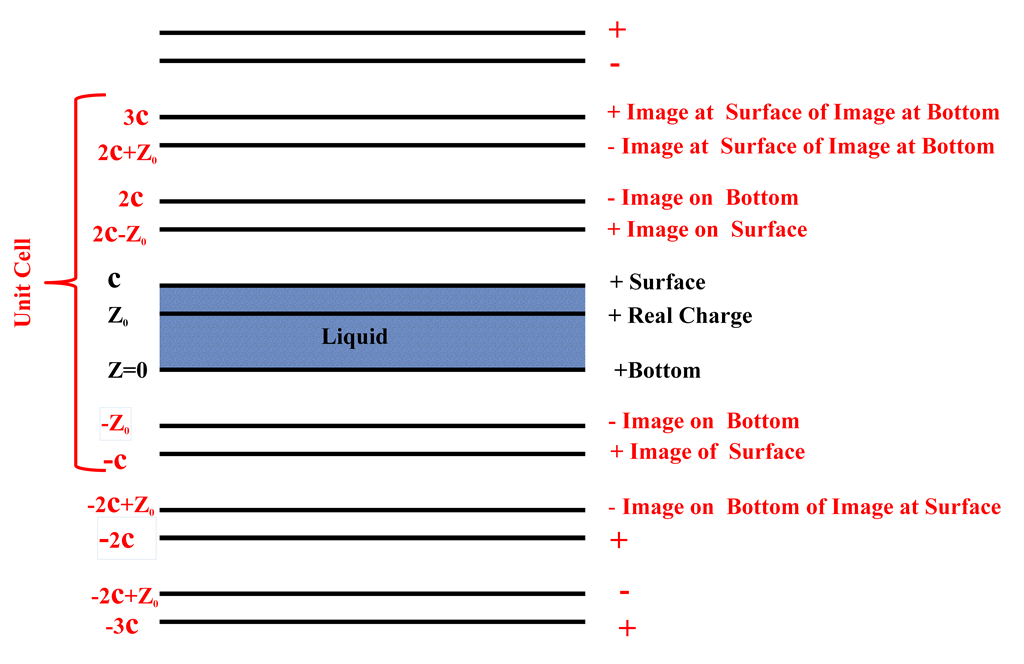
\includegraphics[scale=.6]{../Images/celd1}
	\caption{\emph{Diagram shows that there is a positive (real) plane $ z_0 $, a negative image at $ -z_0 $ below the conductor ($ z = 0 $) and its images are a positive plate at $ 2c-z_0 $ and a negative plate at $ 2c + z_0 $, the image is repeated vertically with the period $ L_z = 4c $}}
		\label{fig:Celda1}
\end{figure}
In Fig. \ref{fig:Celda1} it is observed that there is a positive (real) plane $ z_0 $, a negative image at $ -z_0 $ below the conductor ($ z = 0 $) and its images are a positive plate at $ 2c-z_0 $ and a negative plate at $ 2c + z_0 $. Also, the image is repeated vertically with the period $ L_z = 4c $. Therefore, the equation \ref{Eq:EC11} would be rewritten, like this
 \begin{eqnarray}\label{Eq:EC1}
 \nonumber\phi(\vec{r}) = K+\dfrac{8\pi q}{A} \displaystyle\sum_{n} -\bigg(\abs{z-z_0-nL_z}-\abs{z+z_0-nL_z}-\abs{z+2c+z_0-nL_z}+\abs{z-2c-z_0-nL_z}\bigg) +\\ \nonumber \dfrac{1}{G}\displaystyle\sum_{\vec{G}}\bigg( \displaystyle\sum_{n} \bigg( e^{-\abs{z-z_0-nL_z}} +e^{-\abs{z+z_0-nL_z}}-e^{-\abs{z+2c+z_0-nL_z}}-e^{-\abs{z-2c-z_0-nL_z}}  \bigg)\bigg)\cos(G_x x_0) \cos(G_y y_0) e^{i \vec{G} \cdot \vec{r}}\\
\end{eqnarray}
The constant K is chosen thus $ \phi (z = 0) $, substituting in Eq. (\ref {Eq:EC1}) and after factoring $ e^{- nGL_Z} $ we are explicitly left with the geometric sum over $n$
 {\small
 \begin{eqnarray}
 \nonumber\phi(\vec{r}) = K+\dfrac{16\pi q}{A} \bigg(z+z_0  + \displaystyle\sum_{\vec{G}}\dfrac{1}{G} \bigg(e^{-Gz_0} \sinh(Gz)+e^{-Gz_0(2c_z)} \sinh(Gz_0) -e^{-2Gc} \sinh(Gz) \sinh(Gz_0) \\ \nonumber \dfrac{1+\cosh(2Gc)}{\sinh(2Gc)} - e^{-2Gc}\cosh(2Gc) \sinh(Gz_0)   \bigg) \cos(G_x x_0) \cos(G_y y_0) e^{i \vec{G} \cdot \vec{r}}   \bigg)\\
 \end{eqnarray}
}
Evaluating for $ z = 0 $
 \begin{eqnarray}\label{Eq:EC2}
\nonumber\phi(x, y, 0) = K+\dfrac{16\pi q}{A} \bigg(z_0  + \displaystyle\sum_{\vec{G}}\dfrac{1}{G} \bigg(e^{-2Gc} \sinh(Gz_0)-e^{-2Gc} \sinh(Gz_0)   \bigg) \cos(G_x x_0) \cos(G_y y_0) e^{i \vec{G} \cdot \vec{r}}\bigg) =\\ \nonumber = K+\dfrac{16\pi q}{A} \\
\end{eqnarray}
Independent of $ x $ and $ y $ to configure
 \begin{eqnarray}
 K=\dfrac{16\pi q}{A}
\end{eqnarray}
I can further simplify Eq. (\ref {Eq:EC2}) to get,
 \begin{eqnarray}
\nonumber\phi(\vec{r}) = \dfrac{16\pi q}{A}\bigg( z  + \displaystyle\sum_{\vec{G}}\dfrac{\sinh(Gz_0)}{G} \bigg(e^{-Gz_0} -e^{-3Gc} \dfrac{\cosh(Gc)\sinh(Gz_0)}{\sinh(2Gc)}   \bigg) \cos(G_x x_0) \cos(G_y y_0) e^{i \vec{G} \cdot \vec{r}}  \bigg)\\
\end{eqnarray}
I am sure it is correct. Then it goes to zero at $ z = 0 $. The term with c disappears if $ c \longrightarrow \infty $. The sum converges when $ G \longrightarrow \infty $ if $ z <z_0 <c $ and diverges to $ z \longrightarrow z_0 $. So it seems ready for calculation.
The normal component of the field is
\begin{eqnarray}
\nonumber E_\perp = -\dfrac{16\pi q}{A}\bigg( 1  + \displaystyle\sum_{\vec{G}}\dfrac{1}{G} \cosh(Gz)\bigg(e^{-Gz_0} -e^{-3Gc} \dfrac{\cosh(Gc)\sinh(Gz_0)}{\sinh(2Gc)}   \bigg) \cos(G_x x_0) \cos(G_y y_0) e^{i \vec{G} \cdot \vec{r}}  \bigg)\\
\end{eqnarray}
And the current density is for any $ z $, for our calculation we choose that $ z = 0 $
\begin{eqnarray}\label{Eq:J}
\nonumber J_\perp = -\dfrac{I}{ab}\bigg( 1  + \displaystyle\sum_{\vec{G}}\dfrac{1}{G} \cosh(Gz_0) \bigg(e^{-Gz_0} -e^{-3Gc} \dfrac{\cosh(Gc)\sinh(Gz_0)}{\sinh(2Gc)}   \bigg) \cos(G_x x_0) \cos(G_y y_0) e^{i \vec{G} \cdot \vec{r}}  \bigg)\\
\end{eqnarray}
Integrating on the surface of the sample is obtained $I_{nm} =\int^{a}_0 dx \int^{b}_0 dy \ \ e^{i\vec{G}\vec{r}}$
\begin{eqnarray}
\nonumber I_{nm}=\dfrac{1}{G_x G_y} (e^{-iG_xa}-1) (e^{-G_y b}-1) \\ I_{nm}=\dfrac{ab}{nm \pi^2} ((-1)^n-1-1)(-(1)^m-1-1)
\end{eqnarray}
Using the factor of the reciprocal vector in this way $ \vec {G} = \bigg (\dfrac{\pi}{a} n, \dfrac{\pi}{b} m \bigg) $,
however, as all the coefficients of $ e^{- i \vec{G} \vec{r}} $ in \ref{Eq:J} they are even in $ \vec{G} $ and the integral is odd in n and m, only the constant term taxpayer to the integrated current
\begin{eqnarray}
\nonumber I^{nm} =\int \vec{J} dx  dy =-\int \vec{J}_\perp dx  dy=\dfrac{I}{ab}\int dx \int dy=I
\end{eqnarray}
\subsection{Transfer Matrix Method (TMM)}
One of the methods used for the analysis of photonic crystal structures is the transfer matrix method. We use it to investigate the reflectance of light in a one-dimensional photonic crystal. The electric and magnetic fields within the layers are shown as $E_m$ and $H_m$. Then we can specify the electric and magnetic fields in the air, $ E_0 $ and $ H_0 $, by solving the following matrix equation:
\begin{equation}
\left[
\begin{matrix}
E_{_{0}}\\
H_{_{0}}
\end{matrix}
\right]= \textbf{M}_{_{1}}, \textbf{M}_{_{2}},...,\textbf{M}_{_{N}} \left[
\begin{matrix}
E_{_{m}}\\
H_{_{m}}
\end{matrix}
\right]
\end{equation}
Where N is the total number of layers including the cavity layer and $ M_j $ is the matrix characteristic of the layer $ j $ specified by:
\begin{equation}
\textbf{M}_j = \left[
\begin{matrix}
\cos \delta_j & -\frac{i}{\eta_j} \sin \delta_j \\
-i\eta_j \sin\delta_j & \cos\delta_j
\end{matrix}
\right]
\end{equation}
and
\begin{equation}
\delta_j= \frac{2\pi}{\lambda} \tilde{n}_j d_j \cos \theta_j
\end{equation}
where $ \lambda $ is the wavelength, $ \tilde{n}_{_{j}} = n_{j} - ik_{_{j}}$ is the complex refractive index (CRI) of the layer, $ d_j $ is the thickness of the layer, and $ \theta_j $ is the angle of refraction of light in the $ j $ layer. The parameter $ \eta_ {j} $ for layer j is defined as:
\begin{equation}\label{Eq:Mt1}
\eta_j=\sqrt{\frac{\epsilon_0}{\mu_0}}\tilde{n}_j cos\theta_j \hspace{1cm} (TE \ \ mode)
\end{equation}
y
\begin{equation}\label{Eq:Mt2}
\eta_j=\sqrt{\frac{\epsilon_0}{\mu_0}} \frac{\tilde{n}_j}{cos\theta_j} \hspace{1cm} (TM \ \ mode)
\end{equation}
where $ \epsilon_0 $ and $ \mu_0 $ are permittivity and free space permeability, respectively. The transfer matrix of all the photonic crystal is given by:
\begin{equation}
\textbf{M}=\textbf{M}_1,\textbf{M}_2,...,\textbf{M}_N= \left[
\begin{matrix}
m_{11} & m_{12} \\
m_{21} & m_{22}
\end{matrix}
\right]
\end{equation}
We can write the reflection and transmission coefficients in a one-dimensional photonic crystal nanocavity as:
\begin{equation}
r=\frac{\eta_0(m_{11}m_{12}\eta_m) -(m_{21}+m_{22}\eta_m)}{\eta_0(m_{11}m_{12}\eta_m) -(m_{21}+m_{22}\eta_m)}
\end{equation}
end
\begin{equation}
t=\frac{2\eta_0}{\eta_0(m_{11}m_{12}\eta_m)+(m_{21}m_{22}\eta_m)}
\end{equation}
where $ \eta_0 $ and $ \eta_m $ are parameters for air and outlet layers, respectively (as defined in equations \ref{Eq:Mt1} or \ref{Eq:Mt2}). Furthermore, the reflectivity R and transmittance T of the entire photonic crystal nanocavity is given by:
\begin{equation}
R=|r|^{2}
\end{equation}
y
\begin{equation}
T=\frac{\eta_m}{\eta_0}|t|^{2}
\end{equation}
\section{Experimental Details}
\begin{figure}[H]
	\centering
	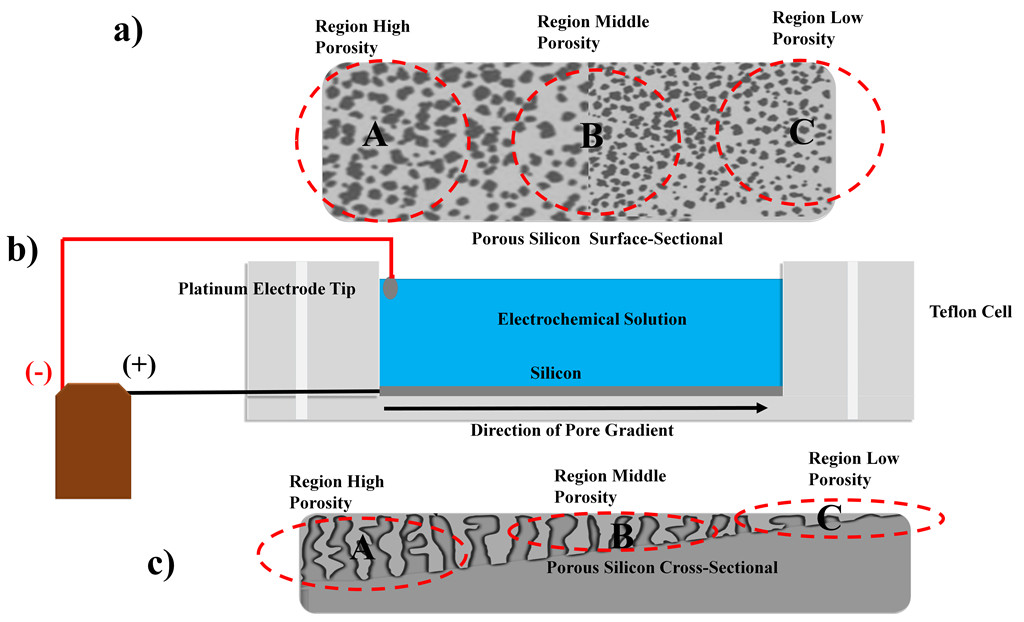
\includegraphics[scale=0.6]{../Images/DE1}
	\caption{\emph{Schematic of the experimental set-up for fabrication of porous silicon with GRIN. a) Represents an outline of the surface section, divided by three regions A, B and C, corresponding to High, Medium and Low Porosity respectively. b) It is the diagram of the electrochemical cell with its parts: silicon wafer, Teflon cell, platinum point electrode, Electrochemical Aqueous solution and the connection of the circuit with the cathode and anode. c) It is a schematic drawing of the Cross section of the electrochemically attacked porous silicon seen in three different regions as mentioned above. }}.
	\label{fig:DE1}
\end{figure}
In the Fig. \ref{fig:DE1} a shows schematic representation of the experimental setup where porous silicon can be manufactured with GRIN, taking into account the considerations of the electrode as tip, the rectangular cell and the sample (silicon wafer) with the largest rectangular attack area.
In Fig. \ref{fig:DE1} a) we draw an outline of the surface section, divided by three regions A, B and C, dependes in therir porosity i.e., High, Medium and Low Porosity. All this corresponding to  expected to be obtained in the experiments. Fig. \ref{fig:DE1} b) the scheme shows the electrochemical cell with its parts: silicon wafer, teflon cell, platinum point electrode, electrochemical Aqueous Solution and the connection of the circuit with the cathode and anode. Finally, Fig. \ref{fig:DE1} c) it is a schematic drawing of the Cross section of the electrochemically attacked porous silicon seen from three different regions as mentioned above. In section 3.1 we give the details used to carry out our experiments.

\subsection{Fabrication of Porous Silicon Monolayers GRIN}
Some of the simulated photonic structures were made by electrochemical anodization on an oriented (100) p-type crystalline Si wafer (resistivity 0.002 - 0.005 $ \Omega \cdot cm $), under galvanostatic conditions. The electrochemical anodization process was performed at room temperature, with an electrolytic mixture of aqueous hydrofluoric acid (HF) (concentration: 48 $ \% $ wt), glycerol (purity: 99.8 $ \% $ wt) and ethanol (purity: 99.9 $ \%$ wt ) in 3: 7: 1 volume ratio, respectively. After the anodizing process, the samples are rinsed with ethanol (purity: 99.9 $ \% $  wt). The layout of the cell used is as seen in Fig. \ref{fig:DE1} b), with an area of $ 1,206 \ \ cm^2 $ (this is the area attacked in the process), has a rectangular shape ($ 0.62 \ \ cm \times 2.03 \ \ cm $)  so that the current densities  that attacks has a lateral gradient with a greater surface area. They were manufactured with a fixed current of $ 5 \ \ mA $ to generate different current densities ranging from $ 6  $ to $ 2.5 \ \ mA / cm^2 $. Similarly, we use the current from $ 40 \ \ mA $ to generate $ 50 $ to $ 20 \ \ mA / cm ^ 2 $. The cathode is made of a platinum wire that was arranged in the form of a tip with an approximate diameter of ($ 0.5 \ \ mm $).
\subsection{Reflectance Measurement}
In the experiemental parte the reflectivity measurements were carried out with a Perkin Elmer Lambda 950 UV-Vis-NIR spectrophotometer. To calculate the complex refractive index $ \tilde{n}_{_{PSi}} = n_{_ {PSi}} - ik_{_{PSi}} $ of a porous layer with homogeneous porosity and thickness with smooth interfaces to throughout the entire structure, the more suitable is the adjustment procedure of the experimental reflectance or transmittance spectrum, this is for the theoretical part. In the case of the reflectance spectrum. The corresponding theoretical calculations were carried using procedure for single  smooth layer (monolayer).
 \begin{eqnarray}\label{Eq:ECMR}
R=\dfrac{r _ {_ {01}}r _ {_ {12}} e^{-2i\delta}}{1+r _ {_ {01}}r _ {_ {12}} e^{-2i\delta}}
\end{eqnarray}
where $ r_{_ {01}} $ y $ r_{_ {12}} $ are the Fresnel reflectance coefficients at the interfaces $aire/PSi$ y $PSi/c-Si$ which are defined in terms of their complex refractive index ($\tilde{n}_{_ {1}} $, $\tilde{n}_{_ {2}} $ y $ \tilde{n}_{_ {3}} $), for them $r_{_{ij}}=(\tilde{n}_{_{i}}\cos\theta_i-\tilde{n}_{_{j}}\cos\theta_j)/(\tilde{n}_{_{i}}\cos\theta_i+\tilde{n}_{_{j}}\cos\theta_j)$, ($j=i=0,1,2$), whilst $\delta=2\pi d/\lambda\sqrt{\tilde{n}^2_{_{2}}-\tilde{n}^2_{_{1}}\sin \theta_1}$.
 To adjust the reflectance spectrum, the layer thickness is an input parameter in the Eq.\ref{Eq:ECMR}. The advantage of this method is the possibility of taking into account the interface roughness effect by including the Davies-Bennett factor in the coefficient of each Fresnel \cite{I17, I18, I19}, which represents the roughness of a Gaussian distribution.
\subsection{Morphological studies}
The morphologies of the etched porous layers (cross-sectional) was observed using SEM Hitachi SU1510 scanning electron microscopes (Hitachi High Technologies Canada, Inc., Toronto, Canada), the thickness  and porosity  of each fabricated  film was measured.
 \subsection{Refraction Indices Monolayer of Porous Silicon GRIN }
Through the electrochemical anodization of c-Si wafers, Psi monolayers were obtained. For the refractive index of each monolayer Psi calcalated by ussing  Bruggeman effective medium theory, as we consider that we have a homogeneous medium associated with effective dielectric function \cite{I20}. This effective dielectric function is related to the dielectric functions of the two media, consisting of two materials (air and silicon), where it is assumed that all the pores or islands of the bulk material experience an average electric field; the equation is expressed as follows:
 \begin{eqnarray}\label{Eq:Brugg}
 p\dfrac{\varepsilon_{_{air}}-\varepsilon_{_{PSi}}}{\varepsilon_{_{air}}+\varepsilon_{_{PSi}}}+(1-p)\dfrac{\varepsilon_{_{Si}}-\varepsilon_{_{PSi}}}{\varepsilon_{_{Si}}+ \varepsilon_{_{PSi}}}
 \end{eqnarray}
 where $ p $ is the volume fraction of air within the PSi layer (porosity); $\varepsilon_{_{air}}$ is the dielectric function of air; $\varepsilon_{_{Si}}$ is the dielectric function of c-Si, and $\varepsilon_{_{PSi}}$ represents the dielectric function of PSi. The dielectric function is a complex number and is related to the complex refractive index ($\tilde{n} = n - ik$), which is made up of real and imaginary parts, as follows $\varepsilon=\tilde{n}^2$. Its real part ($ n $) represents the ordinary refractive index when no light absorption occurs. The imaginary part ($ k $) is known as the extinction coefficient. The extinction coefficient determines the absorption rate in the medium \cite{I21}. Porosity can be estimated using the Bruggeman approximation, from Eq. \ref{Eq:Brugg} provided that the dielectric functions of each component (air and c-Si) are known.

 \subsection{Fabrication  of Microcavities of Porous Silicon GRIN }
 A conventional way to fabricate the porous silicon microcavity (MC) is a defect with a mode located between two DBRs (Distributed Bragg Reflector). Alternate layers of high refractive index (H) and low (L) refractive index are obtained, satisfying the Bragg condition $n_{_{i}}d_{_{i}}=\frac{\lambda_{_{c}}}{4}$  where $ i = H, L $. The defect must meet the condition  $n_{_{L}}d_{_{L}}=\frac{\lambda_{_{c}}}{2}$, and the MC has the following sequence: $$ (HL)_6 HH (LH )_6 $$
 Initial data for conventional design we use $\lambda_{_{c}}= 0.67 \mu m$, $n_{_{H}} =2,6$, $P_{_{H}} =0.46$, $d_{_{H}}=0.066 \mu m  $, $t_{_{H}}=35 s  $ and for $n_{_{L}}= 1,4$,  $P_{_{L}} =0.75$, $d_{_{L}}=0.117 \mu m  $, $t_{_{L}}=11 s  $. All of this data is for the $ 0 $ point of the sample that is located at one end of the sample just below the tip counter-electrode.\\
 Our proposal for the fabrication of porous silicon GRIN microcavities uses the same conditions for fabrications of porous silicon GRIN monolayers as in section 3.1, and taking the conventional data mentioned above. The porous silicon microcavities (PSiMC) with gradient refractive index (GRIN), were manufactured with different current densities ranging from $ 6 $ to $ 2.5 \ \ mA / cm ^ 2 $ for a current of $ 5 \ \ mA $, with high refractive index $n_{_{H}} \sim 2,761 $ to $ 2,808 $ and porosities from $ 0.44 $ to $ 0.39 $. Also for $ 50  $ to $ 20 \ \ mA / cm ^ 2 $, current of $ 38 \ \ mA $, for low refractive index $n_{_{L}}\sim 1,448 $ to $ 2,267 $ and with the corresponding  porosities of $ 0.75 $ to $ 0.64 $. Using our calibration ratio to design GRIN structures,  the corresponding current density for each measurement point.

\section{Discussion and Results}
\subsection{Simulation of the EMPCGRIN model}
 To test the developed  idea in the theoretical section, we find a relation of the tip of the counter electrode that acts similarly as a point charge and the current density for a geometry in an electrolytic box and solve the electrostatic equations with suitable boundary conditions. Resulting in an electrostatic model for photonic crystals with a refractive index with gradient (EMPCGRIN).
\begin{figure}[H]
	\centering
	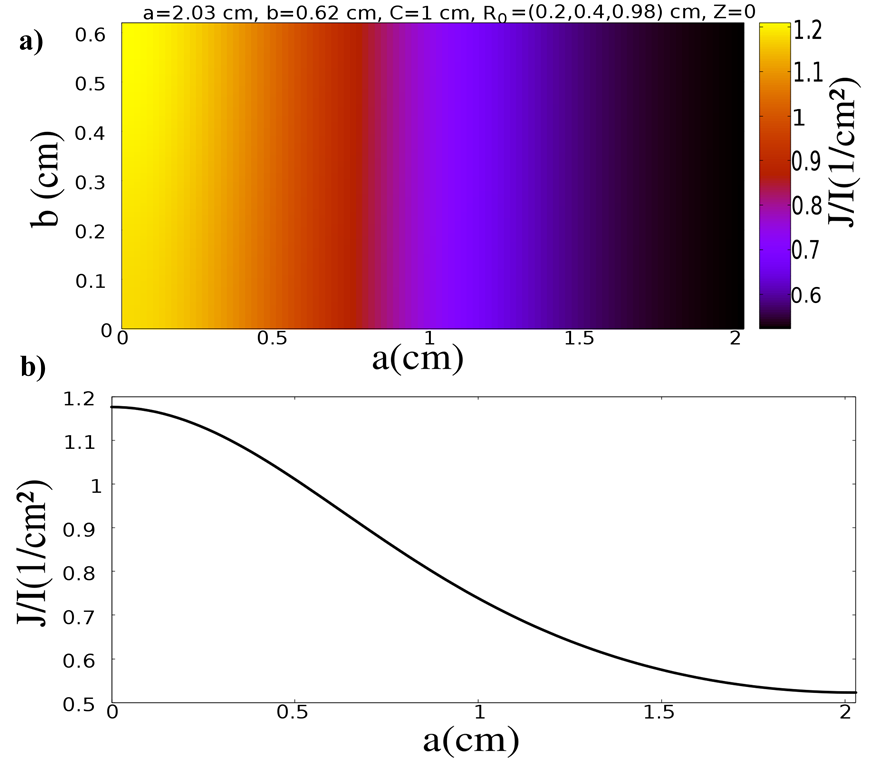
\includegraphics[scale=0.7]{../Images/G123}
	\caption{\emph{ Simulation to calculate the current density in a structure with gradient refractive index (GRIN) produced by electrochemical attack on crystalline silicon to produce porous silicon (PSi), with a current density profile $ J (mA / cm ^ 2 ) $ normalized with the electric current $ I (mA) $, we have $ J / I \sim 0.5 \ \ a \ \ 1.2 (cm^{-2}) $, for a cell of $ a = 2.03 \ \ cm $ y $ b = 0.62 \ \ cm $, with an electrode height $ Z_0 = 0.96 \ \ cm $} Eq. (\ref{Eq:J})}.
		\label{fig:DR1}
\end{figure}
We consider Fig. \ref{fig:DR1} which come from solving Eq. (\ref{Eq:J}), calculating the current density as a function of the rectangular cell area of $1,206 \ \ cm^2 $,  the programming with the PERL PDL package and corresponding graph in gnuplot. We optimize the appropriate values so that our current density adequately attacks crystalline silicon, giving the gradient effect. We use as length $a = 2.03 \ \ cm $ and width $b = 0.62 \ \ cm $ the height of the solution is $ c = 1 \ \ cm $ and we could locate the tip of the electrode at $ R_0 = (X_0 = 0.2 , \ \ Y_0 = 0.4 \ \, Z_0 = 0.96) \ \ cm $ and evaluated at the surface on the silicon interface, in the plane $ Z = 0 $. In this same Figure \ref{fig:DR1}, we obtain a current density profile $ J (mA / cm^2) $ normalized with the electric current $ I (mA) $, we have $ J / I \sim 1.2 \ \ a \ \ 0.5 (cm ^{-2}) $, as we see in Fig. \ref{fig:DR1} a) an effect that happens on the surface of the sample, a change of contrate due to the different densities of attacked currents. We see the decay behavior that the profile has as Fig. \ref{fig:DR1} b) which is a cut on the axis of $ a $. When we vary the currents we can observe the behavior of changes in the normalized current density, with the data obtained through the simulation we could have a better optimization in the design of porous silicon proposing a new and novel experimental arrangement, in the same way we can give ourselves an idea by means of the graph of how the attack would be and the formal side of the pores in the silicon.

\subsection{Monolayers GRIN Porous Silicon }
\begin{figure}[H]
	\centering
	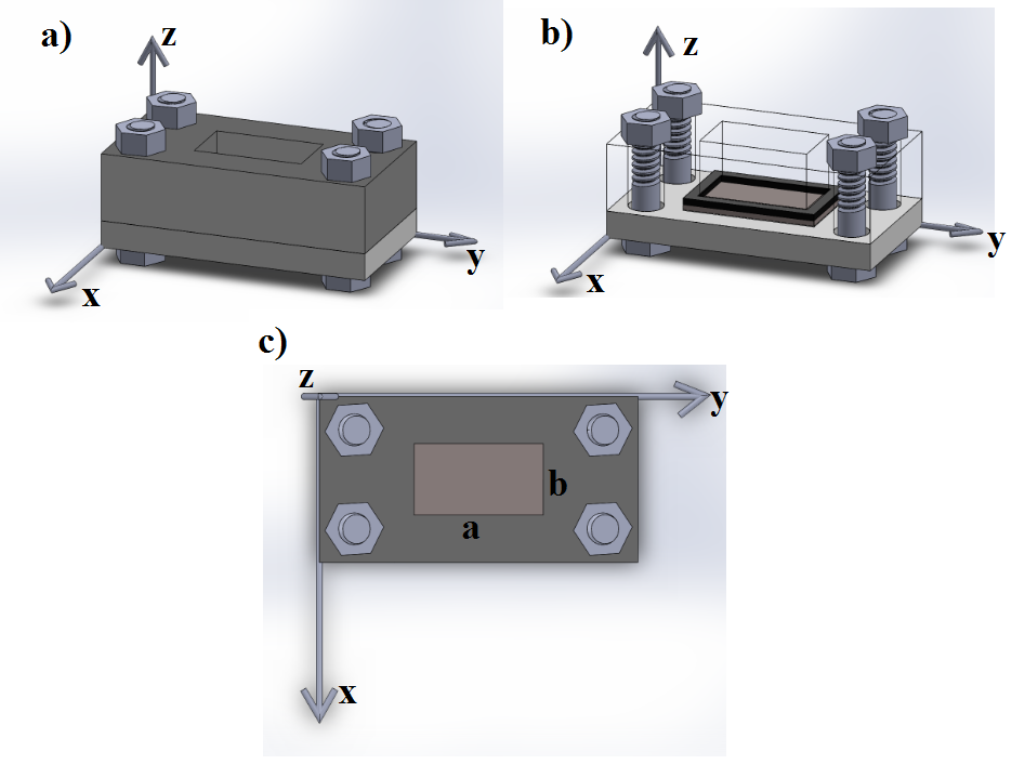
\includegraphics[scale=.3]{../Images/celdan2}
	\caption{\emph{ Mechanical 3D modeling, design of the electrochemical cell where we can see the shape of a prism giving the required and necessary data for the experiments. The design of the cell used is $ 1,206 \ \ cm ^ 2 $ (this is the area attacked in the process), the area attacked is rectangular ($ 0.62 \ \ cm \times 2.03 \ \ cm $) and a height ( $ 1.2 \ \ cm $) a) Complete cell b) Cell without top cover and c) Top view}}
	\label{fig:por1}
\end{figure}
We can see in Fig. \ref{fig:por1}, 3D modeling the mechanical design for the electrochemical cell  better optimization in manufacturing silicon pores where we can see the shape of a prism giving the required data. The design of the cell used is $ 1,206 \ \ cm ^ 2 $ (this is the area attacked in the process), the area attacked is rectangular ($ 0.62 \ \ cm \times 2.03 \ \ cm $) and a height ( $ 1.2 \ \ cm $), all this in order to optimize our experiments adjusted to all the needs that this required.
\begin{figure}[H]
	\centering
	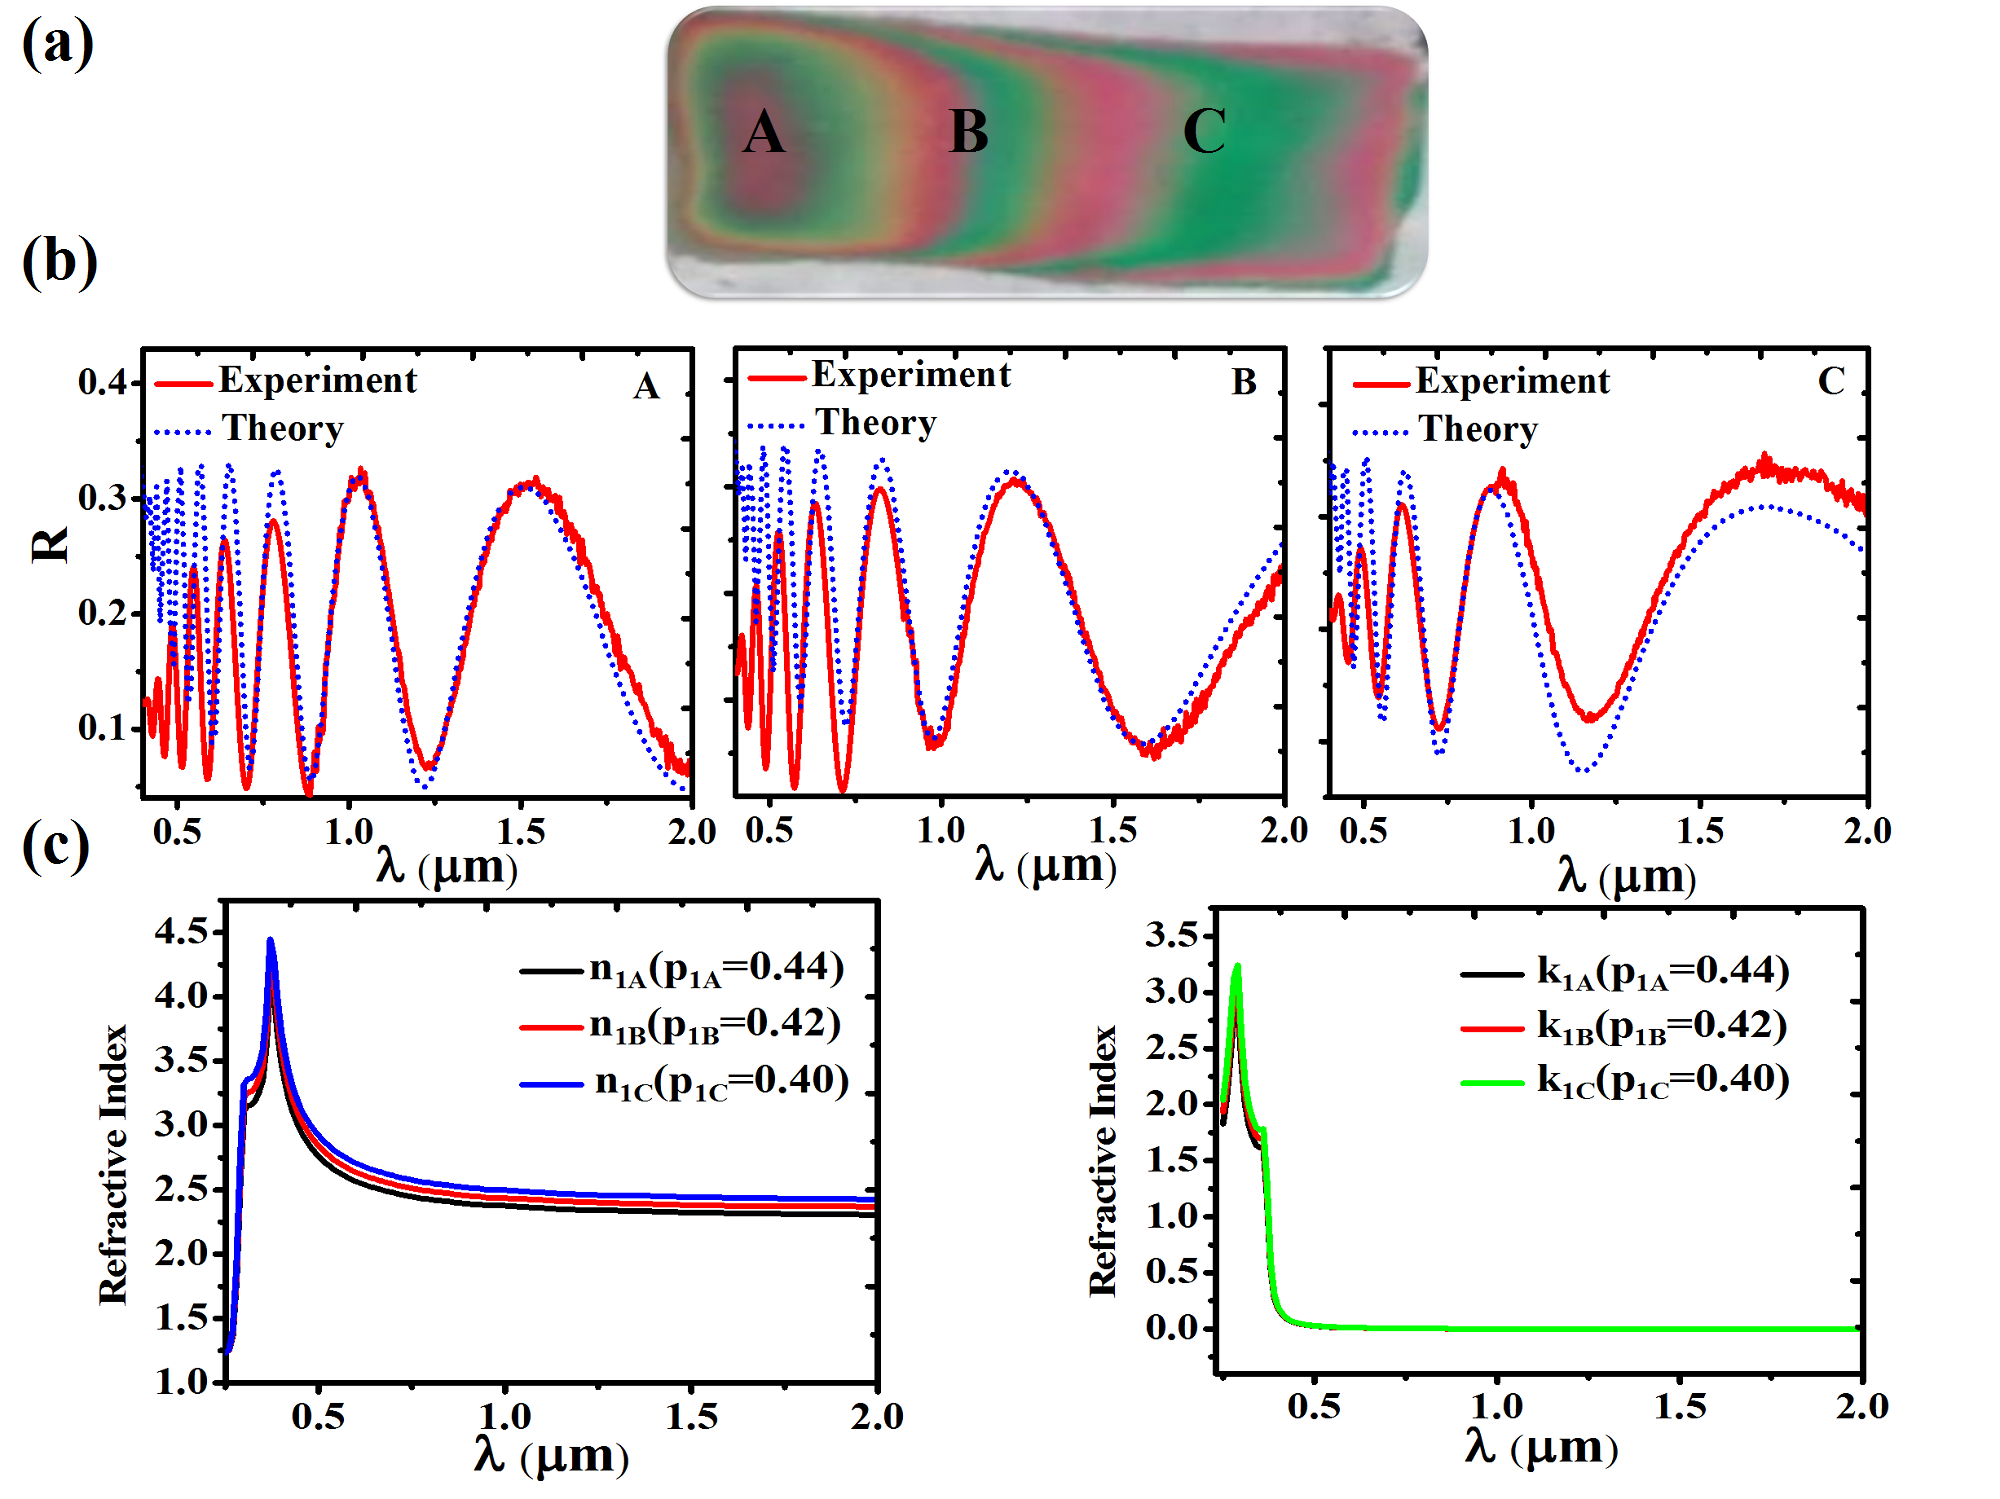
\includegraphics[scale=.5]{../Images/SPgrin51}
	\caption{\emph{a) Silicon sample attacked with an electrolytic mixture of aqueous hydrofluoric acid (HF) (concentration: 48 $ \% $  wt), glycerol (purity: 99.8 $ \% $  wt) and ethanol (purity: 99.9 $ \% $  wt ) in 3: 7: 1 volume ratio, respectively. Obtaining a monolayer of porous Silicon with GRIN G1 with an initial current of G1 (5 mA), with an attack time of 600s. Three different locations are considered, denoted as follows, A (0.3cm) and B (0.8cm) and C (1.7cm). b) Reflectance measurements to know the optical properties at each of the points and the adjustments that were produced by means of the equation \ref{Eq:ECMR}. c) We have the indices of refraction of the complex porous silicon GRIN, where we calculate the real and imaginary part by means of the equation \ref{Eq:Brugg}. for different porosities at each point, A (P = 0.44), B (P = 0.42) and C (P = 0.40) } }
	\label{fig:DR3}
\end{figure}
 The Fig. \ref{fig:DR3} a) three locations at different points are considered, denoted as follows, $ A (0.3 \ \ cm) $ and $ B (0.8 \ \ cm) $ and $ C (1.7 \ \ cm) $, from the sample of PSi GRIN $ G1 (I = 5 mA) $. Also the Fig. \ref{fig:DR3}. b), we have the reflectance measurements to know the optical properties and the adjustments that were produced by means of the equation \ref{Eq:ECMR}. In the Fig. \ref{fig:DR3} c) are indices of refraction of the porous silicon complex GRIN, where we calculate the real and imaginary part by means of Eq. \ref{Eq:Brugg} for different porosities at each point, $ A (P = 0.44) $, $ B (P = 0.42) $ and $ C (P = 0.40) $. Location $ A $ is closest to the electrode, while location $ C $ is furthest to the other end of the sample. Since the current density is applied from one end, the field lines attack the sample laterally to the silicon wafer, in the present configuration, an assembly was made based on the simulated data shown in Fig. \ref{fig:DR1} the experimental part was taken a platinum electrode covering its surface, leaving only a very small area, as if it were a tip. The electrochemical reaction takes place when we apply currents from an anode end (electrode tip) to the silicon substrate (resistivity $ 0.002 - 0.005  \Omega \cdot cm $), through an electrolyte forming a current circuit. The reflectance spectra of the newly recorded G1 samples measured at points $ A (0.3 \ \ cm) $ and $ B (0.8 \ \ cm) $ and $ C (1.7 \ \ cm) $ are presented in Fig. \ref{fig:DR3} b), a numerical reflectivity adjustment was performed using the transfer matrix method for the case of a porous monolayer in Si. It should be noted that the adjustment made was considered a spectral range of the wavelength of the experimental reflectivity spectra for which the silicon can be considered the complex index and thus find the refractive index of the complex porous silicon with the purpose of determining the porosity and the experimental physical thickness (nm) by means of the SEM. The formation of PSi GRIN in the thickness occurs due to the variation in the concentration of the voids available at the Si electrolyte interface, therefore, an increase in the applied lateral current density increases the dimension of the pores and their depth. Thus, the extent of the porous film showing a gradient that can be controlled from the lateral current density.
\begin{figure}[H]
	\centering
	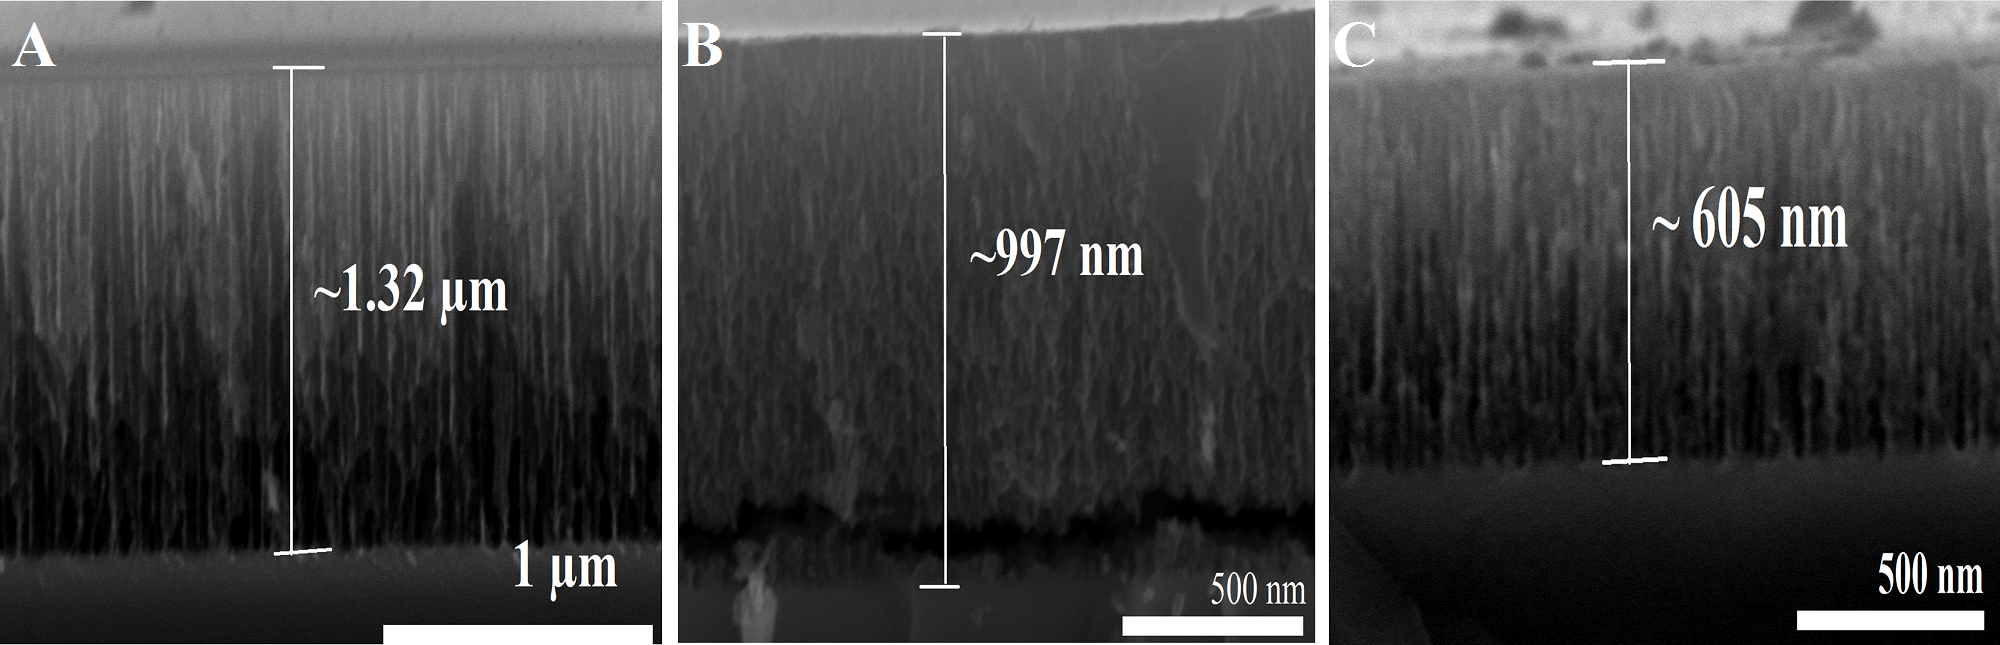
\includegraphics[scale=.5]{../Images/semD11}
	\caption{\emph{Characterization of a monolayer of PSi GRIN G1 with an initial current of $ 5 \ \ mA $, seeing the morphology and depth of the cross section of several SEM micrographs, at different points, $ A (0.3 \ \ cm) $ and $ B (0.8 \ \ cm) $ and $ C (1.7 \ \ cm) $. We can see the sample size for each measurement point, the depth $ d (A) = 1320 \ \ nm $, $ d (B) = 997 \ \ nm $ and $ d (C) = 605 \ \ nm $ } }
	\label{fig:DR4}
\end{figure}
In the Fig. \ref{fig:DR4} shows the cross section views   at points $ A (0.3 \ \ cm) $, $ B (0.8 \ \ cm) $ and $ C (1.7 \ \ cm) $, we can measure the thickness for each point of the sample $ G1 (I = 5 \ \ mA) $, $ d (A) = 1320 \ \ nm $, $ d (B) = 997 \ \ nm $ and $ d (C) = 605 \ \ nm $. Likewise, we could check it for a second sample $ G2 (I = 40 \ \ mA) $, with porosities for each point, $ A (P = 0.76) $, $ B (P = 0.73) $ and $ C (P = 0.68) $ and the depths $ d (A) = 1950 \ \ nm $, $ d (B) = 1690 \ \ nm $ and $ d (C) = 1430 \ \ nm $, designed in the same way as the shows G1, only varying the current taking into account the current density ratio for each point. Apart from that, a structural gradient was formed, along the direction \emph{ a}  of the axis of the $ x $, where the tip of the electrode is near the point $ A $ and away from the point $ C $ of the substrate, using the proposed experimental setup. In addition, it was possible to control the current density based on the position of the sample and the depth, seen in the SEM micrographs.
 \begin{figure}[H]
 	\centering
 	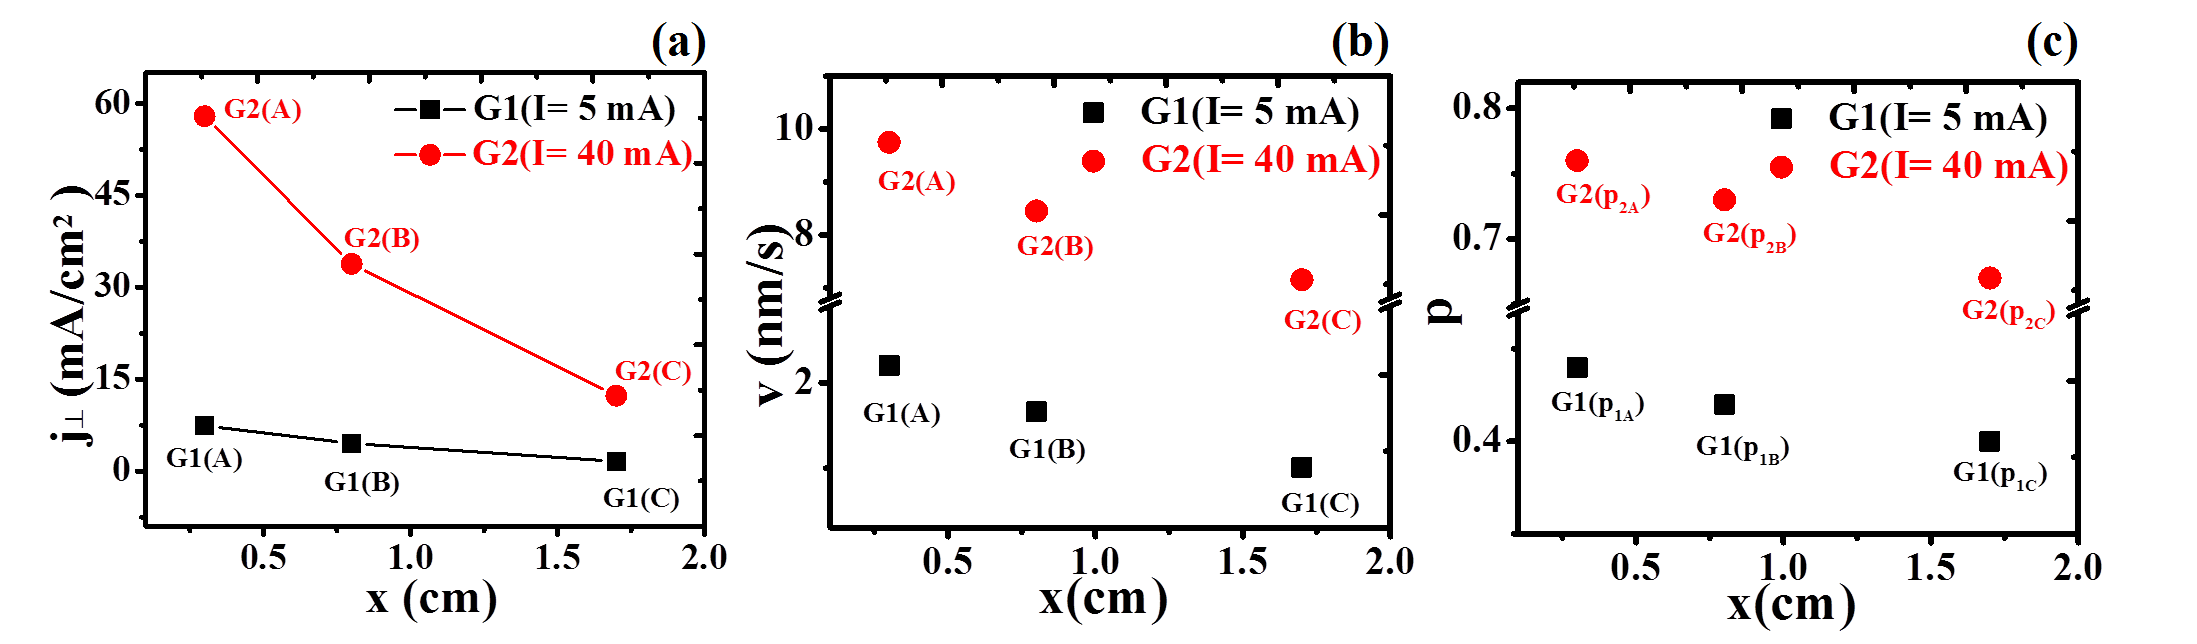
\includegraphics[scale=.7]{../Images/grinJDR}
 	\caption{\emph{a) It is the relation of the current density $ J (mA / cm ^ 2) $ normalized with the electric current $ I (mA) $, we have $ J / I \ sim 1.2 \ \ a \ \ 0.5 ( cm^{-2}) $, when we apply it to two samples $ G1 (I = 5 \ \ mA) $ and $ G2 (I = 40 \ \ mA) $ depending on the axis $ a $ $ (0.1 ... 2.0 \ \ cm) $, measured at points $ A (0.3 \ \ cm) $ , $ B (0.8 \ \ cm) $ and $ C (1.7 \ \ cm) $. b) The attack speed $ v = d (J_i) / t (nm / sec) $, the depths (thickness $ d (J_i) $, $ i = $ $ A (0.3 \ \ cm) $, $ B ( 0.8 \ \ cm) $ y $ C (1.7 \ \ cm)) $ taken in SEM micrographs $ d (J_i) (nm) $ and attack times $ G1 (t = 600 \ \ s) $ y $ G2 (t = 200 \ \ s) $, depending on the axis $ a $ $ (0.1 ... 2.0 \ \ cm) $ } }
 	\label{fig:JDR}
 \end{figure}
In Fig. \ref{fig:JDR} a) It is the relation of the current density $ J (mA / cm ^ 2) $ normalized with the electric current $ I (mA) $, we have $ J / I \ sim 1.2 \ \ a \ \ 0.5 (1 / cm ^ 2) $, when we apply it to two samples $ G1 (I = 5 \ \ mA) $ and $ G2 (I = 40 \ \ mA) $ depending on the axis $ a $ $ (0.1 ... 2.0 \ \ cm) $, measured at points $ A (0.3 \ \ cm) $ and $ B (0.8 \ \ cm) $ and $ C (1.7 \ \ cm) $.
The Fig. \ref{fig:JDR} b) we can calculate the attack speed $ v = d (J_i) / t (nm / s) $, where the depths (thickness $ d (J_i) $, $ i = $ $ A (0.3 \ \ cm) $, $ B (0.8 \ \ cm) $ and $ C (1.7 \ \ cm)) $ taken in SEM micrographs $ d (J_i) (nm) $ and attack times $ G1 (t = 600 \ \ s) $ and $ G2 (t = 200 \ \ s) $, depending on the axis $ a $ $ (0.1 ... 2.0 \ \ cm) $.
\begin{figure}[H]
	\centering
	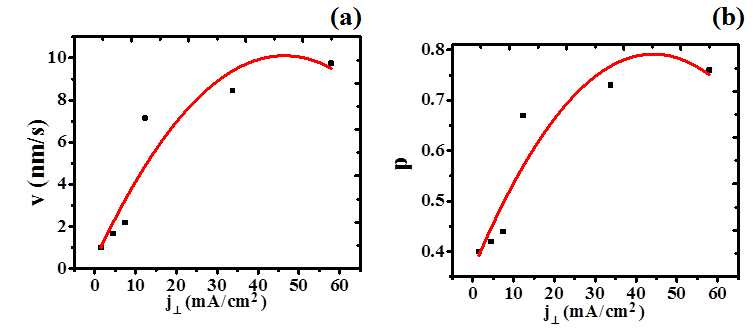
\includegraphics[scale=.6]{../Images/grinJD31}
	\caption{\emph{The relationship of samples $ G1 (I = 5 mA) $ and $ G2 (I = 40 mA) $ were obtained to find: a) Attack speed with current density for each point and b) Porosity as a function of density current. With this we have the calibration curves for the manufacture of any GRIN porous silicon structure   } }
		\label{fig:Indr1}
\end{figure}
Fig. \ref{fig:Indr1} a) explicitly explain the relationships that emerge when designing samples $ G1 (I = 5 mA) $ and $ G2 (I = 40 mA) $. For the first case $ G1 $ the depths ($ 1320 \ \ nm $ to $ 605 \ \ nm $) and the current densities ($ 6 \ \ mA / cm ^ 2 $ to $ 2.5 \ \ mA / cm ^ 2 $), finding the attack speed $ 2.2 \ \ nm / s $ up to $ 1.1 \ \ nm / s $ relation with depth and the time ($ 600 \ \ s $) of exposure of the sample, with the current density . We also find the depth ($ 1950 \ \ nm $ at $ 1430 \ \ nm $) and the current density ($ 50 \ \ mA / cm ^ 2 $ at $ 20 \ \ mA / cm ^ 2 $) as a function of the measurement points of the sample $ G2 (I = 40 mA) $. We were able to obtain the attack speed from $ 9.8 \ \ nm / s $ up to $ 7.1 \ \ m / s $ by relating to depth and time ($ 200 \ \ s $), with current density. Once the thickness of the monolayer and the attack time applied to them are known, calculate the attack speed according to the formula $ v = d / t $, for each of the current densities at the points $ A ( 0.3 \ \ cm) $ and $ B (0.8 \ \ cm) $ and $ C (1.7 \ \ cm) $. Then we fit a function to the attack speed points with the different current densities allowed by the anodizing condition. For a desired thickness $ d (J_i) $, calculate the attack time $ t $ (so, $ t = v / d (J_i) $) and we can design any structure knowing the current density and the attack time. Fig. \ref{fig:Indr1} b) we find a relation of the porosity for each position with its determined current density. Therefore, if it is desired to manufacture a PSi monolayer of a certain porosity with a certain end, it is enough to resort to the graphs of Fig. \ref{fig:Indr1} to determine the corresponding current density, attack speed and consequently the time, obtaining for that monolayer. The importance of the calibration curves is that it allows us to have a relationship of the porosities that can be reached (and by having control over the possible refractive indices) as a function of the current density and to be controlled to control the thickness of the layers that are manufactured, by controlling the attack time for each of the chosen currents.

\subsection{GRIN Porous Silicon Microcavities}
 \begin{figure}[H]
	\centering
	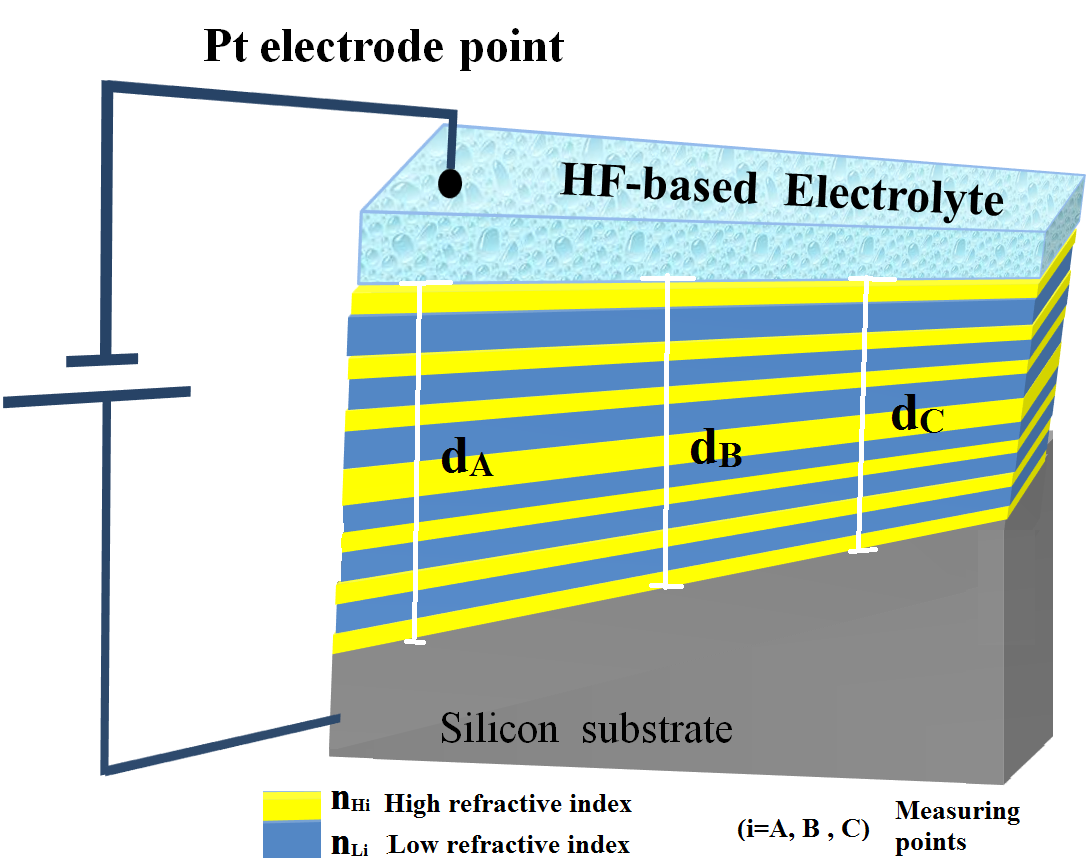
\includegraphics[scale=0.4]{../Images/MicrGrin}
	\caption{\emph{Diagram of a microcavity of porous silicon GRIN. Alternate layers are obtained of high (H) refractive index $n_{_{Hi}}$ and low (L) refractive index $n_{_{Li}}$, where $N_{_{H}}$ is the number of layers for  $n_{_{Hi}}$ and $N_{_{L}}$ is the number of layers for $n_{_{Li}}$. Then,  $d_{_{Hi}}$ is the monolayer thickness of  $n_{_{Hi}}$ at that measurement point and $d_{_{Li}}$ is the monolayer thickness of $n_{_{Hi}}$ at that measurement point. Therefore,  $d_{_{i}}$ is the total thickness calculated for each of the measurements, defining a i = $ A, B, C$. Having the following relationship $d_{_{i}} = (N_{_{Hi}}d_{_{Hi}})+(N_{_{Li}}d_{_{Li}}) + (2d_{_{Hi}})$. }}
	\label{fig:MCGRIN0}
\end{figure}
The Fig. \ref{fig:MCGRIN0} the scheme of  a initially proposed lateral gradient for monolayers should be shown in section 4.2, where we designed an electolytic cell suitable for our experiments and giving us the expected results of the simulation in section 4.1. Now our purpose is to manufacture more complex photonic structures such as the Porous silicon microcavities GRIN, taking into account that we start from having a tip electrode almost on the surface and by making a variation of currents we can achieve the effect of alternating the layers. Alternate layers are obtained of high (H) refractive index $n_{_{Hi}}$ and low (L) refractive index $n_{_{Li}}$, where $N_{_{H}}$ is the number of layers for  $n_{_{Hi}}$ and $N_{_{L}}$ is the number of layers for $n_{_{Li}}$. Then,  $d_{_{Hi}}$ is the monolayer thickness of  $n_{_{Hi}}$ at that measurement point and $d_{_{Li}}$ is the monolayer thickness of $n_{_{Hi}}$ at that measurement point. Therefore,  $d_{_{i}}$ is the total thickness calculated for each of the measurements, defining a i = $ A, B, C$. Having the following relationship $d_{_{i}} = (N_{_{Hi}}d_{_{Hi}})+(N_{_{Li}}d_{_{Li}}) + (2d_{_{Hi}})$.
Initial data for conventional design we use  $\lambda_{_{c}}= 0.67 \ \ \mu m$, $n_{_{H}} =2.6$, $P_{_{H}} =0.46$, $d_{_{H}}=0.066 \ \ \mu m  $, $t_{_{H}}=35 s  $ y para  $n_{_{L}}= 1.4$,  $P_{_{L}} =0.75$, $d_{_{L}}=0.117 \ \ \mu m  $, $t_{_{L}}=11 s  $. All these data are for the point $ 0 $ which is located at one end of the sample just below the tip counter-electrode.
\begin{figure}[H]
 	\centering
 	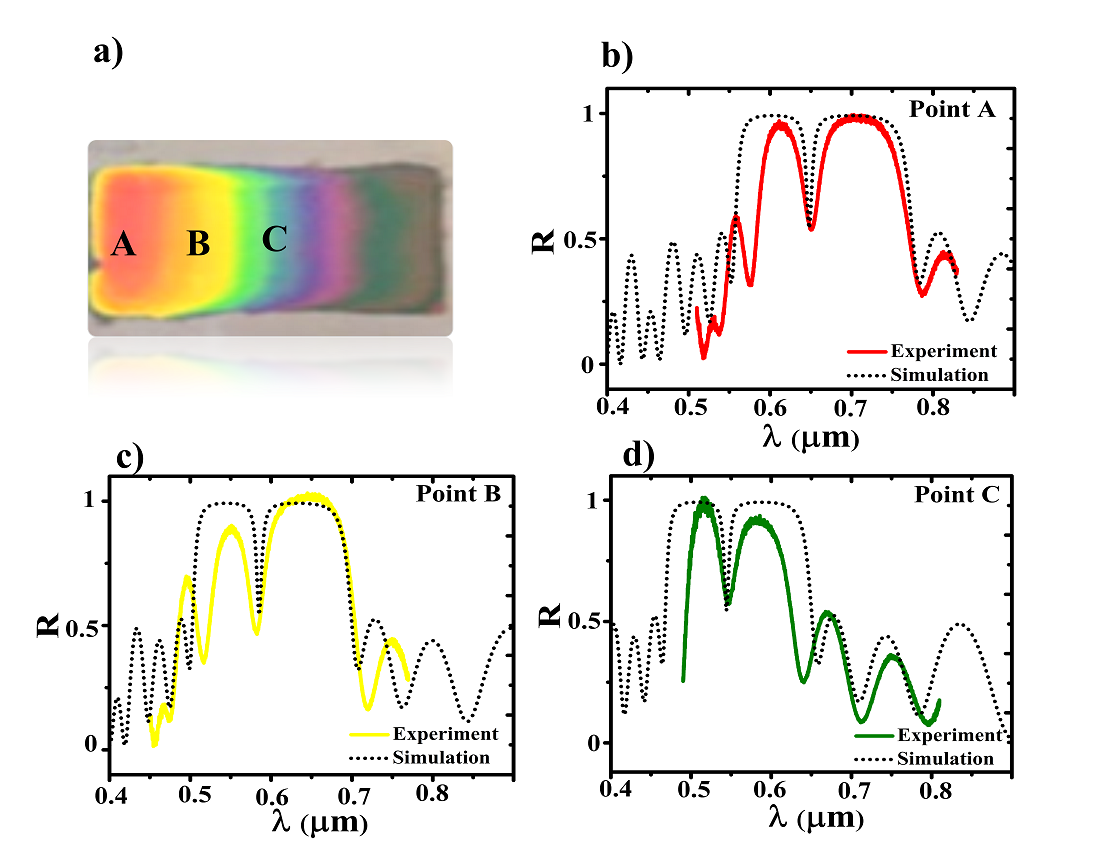
\includegraphics[scale=.5]{../Images/MCGRIN2}
 	\caption{\emph{a) Three locations at different points are considered, denoted as follows, $ A (0.3 \ \ cm) $ and $ B (0.8 \ \ cm) $ and $ C (1.2 \ \ cm) $, from the PSiMCGRIN sample $ GMC $. b) We have the reflectance measurements to know the optical properties with the proposed simulation. We were able to show that in a Porous Silicon GRIN structure, for a microcavity the data is very consistent with the simulation and the experiment, we found the refractive indices and the porosities as a function of the current density at each measurement point, see Table \ref{tabla:1}. }}
 	\label{fig:MCGRIN3}
 \end{figure}

\begin{table}[H]
	\centering
	\begin{tabular}{|c|c|c|c|c|c|c|}
		\hline
		\textbf{Points} & $\lambda_c (\mu m)$ & \textbf{n} & \textbf{k} & \textbf{Porosity} & \textbf{J}$(mA/cm^2)$ & \textbf{t(s)}\\
		\hline
		A(H) & 0.65 & 2.661 & 0.0264 & 0.45 & 5.5 & 35 \\
		\hline
		B(H) & 0.58 & 2.762 & 0.0135 & 0.41 & 4.0 & 35 \\
		\hline
		C(H) & 0.54 & 2.808 & 0.0178 & 0.39 & 3.0 & 35 \\
		\hline
		A(L) & 0.65 & 1.442 & 0.0015 & 0.74 & 44 & 11 \\
		\hline
		B(L) & 0.58 & 2.295 & 0.0091 & 0.68 & 32 & 11 \\
		\hline
		C(L) & 0.54 & 2.302 & 0.001 & 0.64 & 24 & 11 \\
		\hline
	\end{tabular}
	\caption{ \emph{We have different points denoted as follows, $ A (0.3 \ \ cm) $ and $ B (0.8 \ \ cm) $ and $ C (1.2 \ \ cm) $, from the sample of a Porous Silicon Microcavity GRIN  (PSiMCGRIN) $ GMC $. Alternate layers of high refractive index (H) and low refractive index (L) are obtained at each of the measurement points (A, B and C). The refractive indexes of the PSiMCGRIN were considered from the experimental and theoretical values that were obtained for the porosity ($ P = 0.3J^{0.24}$). And we could obtain the attack time with the relation of $ V = 0.53J ^ {0.79} $ where $ t = d / V $.}}
	\label{tabla:1}
\end{table}
In Fig. \ref{fig:MCGRIN3} a) Three locations at different points are considered, denoted as follows, $ A (0.3 \ \ cm) $ , $ B (0.8 \ \ cm) $ and $ C (1.2 \ \ cm) $, from the PSiMCGRIN sample $ GMC $. Likewise, Fig. \ref{fig:DR3} b), we have the reflectance measurements to know the optical properties with the proposed simulation. We can see how from an experimental setup we have some important results as a result of a whole calibration curve suitable for making GRIN porous silicon. The refractive index of the Porous Silicon Microcavities GRIN were considered the experimental and theoretical values obtained for the porosity and the thicknesses shown in Table 1. The porous silicon microcavities (MCSP) with refractive index with gradient (GRIN), were manufactured with different current densities ranging from $ 6 \ \ mA / cm ^ 2 $ to $ 2.5 \ \ mA / cm ^ 2 $ for a current of $ 5 \ \ mA $, for a $t_{_{H}}=35 s $, with a high refractive index $n_{_{H}} \sim$ $ 2,661$ to $ 2,808$ and porosities of $P_{_{H}} \sim$ $ 0.45 $ to $ 0.39 $. Also for $ 44 \ \ mA /cm^2 $ to $ 24 \ \ mA / cm^2 $, current of $ 38 \ \ mA $, using $t_{_{H}}=11 s$  for low refractive index $n_{_{L}}\sim$ $ 1,448 $ to $ 2,267 $ and with porosities of  $P_{_{H}} \sim$ $0.75 $ to $ 0.64 $. The porosity was calculated with the calibration curve exposed in the ($ P = 0.3J^{0.24} $). And the attack time could be obtained with the relation of $ V = 0.53J^{0.79} $ where $ t = d / V $ and the refractive index using the Bruggeman formula. For theoretical values, we use complex refractive indices as free parameters to fit the experimental refractive spectra (Section 4.2).
 \begin{figure}[H]
	\centering
	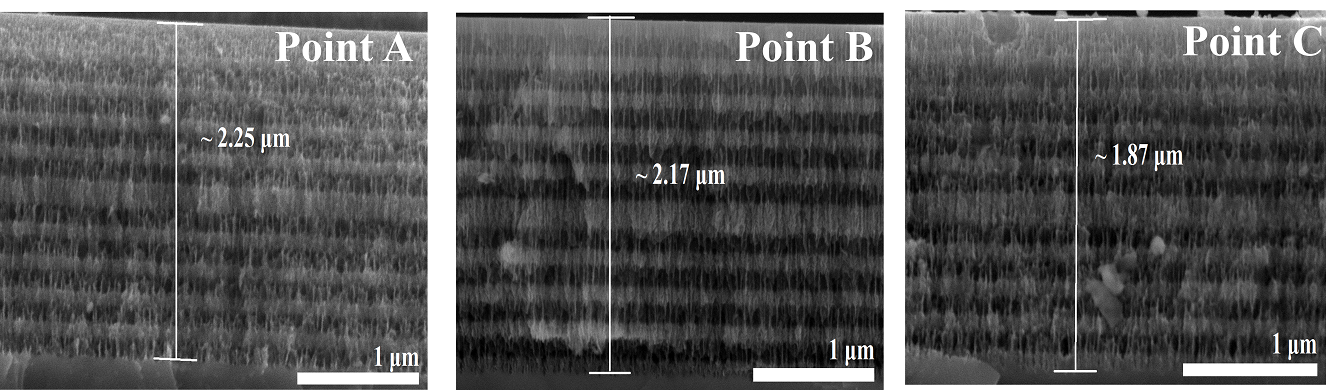
\includegraphics[scale=.5]{../Images/MCGRINSEM}
	\caption{\emph{SEM image of the cross section profile of the microcavities with GRIN. The measured thicknesses of the complete multi-film structures showed good agreement with the simulations taken from $ V = 0.53J ^ {0.79} $ where $d_j=Vt_j$ ($j=H,L$), which are the thicknesses of each of the monolayer of the porous silicon microcavity GRIN at the measurement points and the total thickness we find it as $d_{_{i}} = (N_{_{Hi}}d_{_{Hi}})+(N_{_{Li}}d_{_{Li}}) + (2d_{_{Hi}})$ defining $ i = $ A, B, C. Which resulted in (measured / simulation) $ 2.25 / 2.31 \ \ \mu m $ (for structure at Point A), $ 2.17 / 2.08 \ \ \mu m $ (for structure at point B) and $ 1.87 / 1.65 \ \ \mu m $ (for structure at point C)}}
	\label{fig:MCGRIN4}
\end{figure}

For the Fig. \ref{fig:MCGRIN4} shows the SEM cross-sectional images of the PSi samples used in this work. Relatively small interface roughness and a clear contrast between the high and low porosity of the microcavity measured at different points (A, B and C), showing the change in thickness in each of these. The measured thicknesses of the complete multi-film structures showed good agreement with the simulations taken from $ V = 0.53J^{0.79} $ where $d_j=Vt_j$ ($j=H,L$), which are the thicknesses of each of the monolayer of the porous silicon microcavity GRIN at the measurement points and the total thickness we find it as $d_{_{i}} = (N_{_{Hi}}d_{_{Hi}})+(N_{_{Li}}d_{_{Li}}) + (2d_{_{Hi}})$ defining $ i = $ A, B, C. Which resulted in (measured / simulation) $ 2.25 / 2.31 \ \ \mu m $ (for structure at Point A), $ 2.17 / 2.08 \ \ \mu m $ (for structure at point B) and $ 1.87 / 1.65 \ \ \mu m $ (for structure at point C).
Being able to say that for each measurement point corresponds different calculated current densities, which correspond to different thicknesses at the end of manufacturing, clearly seeing the lateral gradient product of our experiment.


\newpage
\section{conclusion}
The necessary expressions for the potential components were derived, finding a relationship of the tip of the counter electrode that acts similarly as a point charge and the current density for a geometry in a rectangular electrolytic box and we solve the electrostatic equations with suitable boundary conditions. Resulting in an electrostatic model for  Photonics crystals with a refractive index with gradient (EMPCGRIN).
It is the first time that the formalism mentioned here has been applied to find the current density to design porous silicon. The shape of the electrode, the area of the cell produces a visible decrease in the size and density of the pores. Additionally, optimizing the structural properties for a single structure we could have a gradient with different depths, reflactances at differents measurement points. In this way, we were able to simulate the direct relationship of the attack speed with the current density at the points  the samples of interest. At the same time, we developed a characterization between porosity, refractive indices of porous silicon, with the different current densities. And in the end we were able to design and characterize Porous Silicon microcavities with refractive indices with gradients, which for each measurement point correspond to different calculated current densities, which correspond to different thicknesses, clearly seeing the lateral gradient product of our experiment.
\section{Acknowledgments}
% \backmatter
%\nocite{*}
%\bibliographystyle{plain}
%\bibliography{bibliograf�a.bib} %Aqu� ponen el nombre del archivo .bib
\bibliographystyle{unsrt}
 \small{
\begin{thebibliography}{X}
	%forma de biblio es MLA
\bibitem{I1} P. Yeh,\textquotedblleft \emph{Optical Waves in Layered Media} \textquotedblright, 2nd edn. (Wiley-Interscience Publication,
USA, 2005).
\bibitem{I2}Canham, L. 1997.\textquotedblleft \emph{Properties of Porous Silicon} \textquotedblright. Edited by Canham L. DERA, Malvern, UK.
\bibitem{I3}{Beale, M.I.J, J.D Benjamin, M.J Uren, N.G Chew, and A.G Cullis. 1985. \emph{ \textquotedblleft An Experimental and Theoretical Study of the Formation and Microstructure of Porous Silicon.\textquotedblright} J. Crystal Growth 73: 622?36. doi:10.1021/jp0706984. }
\bibitem{I4}Canham, L. T. 1990. \emph{\textquotedblleft Silicon Quantum Wire Array Fabrication by Electrochemical and Chemical Dissolution of Wafers.\textquotedblright} Applied Physics Letters 57 (10): 1046. doi:10.1063/1.103561.


\bibitem{I5} J. D. Joannopoulos et al.,\textquotedblleft \emph{Photonic Crystals: Molding the Flow of Light}\textquotedblright, 2nd edn.
(Princeton University Press, UK, 2008).
\bibitem{I6} E. Yablonovitch, \textquotedblleft \emph{Photonic band-gap structures,}\textquotedblright J. Opt. Soc. Am. B 10, 283-295 (1993)
\bibitem{I7} Ilyas, S., and M. Gal.  \textquotedblleft \emph{ Optical devices from porous silicon having continuously varying refractive index.}\textquotedblright Journal of Materials Science: Materials in Electronics 18.1 (2007): 61-64.
\bibitem{I8} Tran, P. \textquotedblleft \emph{Optical switching with a nonlinear photonic crystal: a numerical study.}\textquotedblright Optics letters 21.15 (1996): 1138-1140.
 \bibitem{I9} Ariza-Flores, A. David, L. M. Gaggero-Sager, and V. Agarwal. \textquotedblleft \emph{White metal-like omnidirectional mirror from porous silicon dielectric multilayers.}\textquotedblright Applied Physics Letters 101.3 (2012): 031119.
\bibitem{I10} Johnson, Steven G., et al.  \textquotedblleft \emph{Linear waveguides in photonic-crystal slabs.}\textquotedblright Physical Review B 62.12 (2000): 8212.

%asimetrica
\bibitem{I101}Collins, Boyce E., et al. \textquotedblleft \emph{ Determining protein size using an electrochemically machined pore gradient in silicon.}\textquotedblright Advanced Functional Materials 12.3 (2002): 187-191.

\bibitem{I102} Khung, Y. L., G. Barritt, and N. H. Voelcker. \textquotedblleft \emph{Using continuous porous silicon gradients to study the influence of surface topography on the behaviour of neuroblastoma cells.}\textquotedblright Experimental cell research 314.4 (2008): 789-800.

\bibitem{I103} Clements, Lauren R., et al. \textquotedblleft \emph{Mesenchymal stem cell attachment to peptide density gradients on porous silicon generated by electrografting.}\textquotedblright physica status solidi (a) 208.6 (2011): 1440-1445.

\bibitem{I104} Wang, Peng-Yuan, et al. \textquotedblleft \emph{Screening the attachment and spreading of bone marrow-derived and adipose-derived mesenchymal stem cells on porous silicon gradients.}\textquotedblright Rsc Advances 2.33 (2012): 12857-12865.

 \bibitem{I11} Canham, L. \textquotedblleft \emph{Properties of Porous Silicon.}\textquotedblright Edited by Canham L. DERA, Malvern, UK. (1997).
 \bibitem{I12} Li, Yang Yang, Peter Kim, and Michael J Sailor.\textquotedblleft \emph{Painting a Rainbow on Silicon A Simple Method to Generate a Porous Silicon Band Filter Gradient}\textquotedblright Physica Status Solidi (a) 1618 (8): 161618. doi:10.1002/pssa.200461200.(2005)
 \bibitem{I13} Khung, Y L, and N H Voelcker. 2009.\textquotedblleft\emph{ Multidirectional Lateral Gradient Films with Position-Dependent Photonic Signatures Made from Porous Silicon.}\textquotedblright Optical Materials 32 (1): 23442. doi:10.1016/j.optmat.2009.07.015.
 \bibitem{I14}  Khung, Y L, G Barritt, and N H Voelcker.  \textquotedblleft \emph{Using Continuous Porous Silicon Gradients to Study the Influence of Surface Topography on the Behaviour of Neuroblastoma Cells.}\textquotedblright Experimental Cell Research 314 (4): 78900. doi:10.1016/j.yexcr.2007.10.015.(2008.)
\bibitem{I15} Collins, B.E., K.-P.S. Dancil, G. Abbi, and M.J. Sailor. 2002.\textquotedblleft \emph{Determining Protein Size Using an Electrochemically Machined Pore Gradient in Silicon.}\textquotedblright Advanced Functional Materials 12 (3): 187. doi:10.1002/1616-3028(200203)12:3,187::AID-ADFM187,3.0.CO;2-E.( 2002.)

\bibitem{I16} Ocier, C. R., Krueger, N. A., Zhou, W. and  Braun, P. V. (2017).\textquotedblleft \emph{Tunable visibly transparent optics derived from porous silicon.}\textquotedblright ACS Photonics, 4(4), 909-914.
%ecuacion
\bibitem{I17} Dariani RS, Ebrahimnasab S (2014). \textquotedblleft \emph{Root Mean Square Roughness of Nano Porous Silicon by Scattering Spectra.}\textquotedblright The
European Physical Journal Plus 129: 129.
\bibitem{I18} Lerondel G, Romestain R (1997).\textquotedblleft \emph{Roughness of the Porous Silicon Dissolution Interface.}\textquotedblright Journal of Applied Physics 81:  61716178.
\bibitem{I19} L�rondel G, Romestain R, Barret S (1997).\textquotedblleft \emph{Quantitative Analysis of the Light Scattering Effect on Porous Silicon
Optical Measurements.}\textquotedblright Thin Solid Films 297: 114?117.

\bibitem{I20} Thei, W. \textquotedblleft \emph{Optical Properties of porous silicon.}\textquotedblright Surf. Sci. Rep. 1997, 29, 91?93.
\bibitem{I21} Van Groesen, E.; Sopaheluwakan, A.; Andonowati, A. \textquotedblleft  \emph{Direct characterization of states and modes in defect grating structures.}\textquotedblright J. Nonlinear Opt. Phys. Mater. 2004, 13, 155173.
% \textquotedblleft \textquotedblright


\bibitem{In} Mazzoleni, C., and L. Pavesi. \textquotedblleft  \emph{Application to optical components of dielectric porous silicon multilayers.}\textquotedblright Applied Physics Letters 67.20 (1995): 2983-2985

\end{thebibliography}
%capitulos1111111111111111111111




\end{document}